\documentclass[a4paper,11pt]{article}
\usepackage{amsmath,amsthm,amsfonts,amssymb,amscd,amstext,vmargin,graphics,graphicx,tabularx,multicol} 
\usepackage[francais]{babel}
\usepackage[utf8]{inputenc}  
\usepackage[T1]{fontenc} 
\usepackage{pstricks-add,tikz,tkz-tab,variations}
\usepackage[autolanguage,np]{numprint} 

\setmarginsrb{1.5cm}{0.5cm}{1cm}{0.5cm}{0cm}{0cm}{0cm}{0cm} %Gauche, haut, droite, haut
\newcounter{numexo}
\newcommand{\exo}[1]{\stepcounter{numexo}\noindent{\bf Exercice~\thenumexo} : \marginpar{\hfill /#1}}
\reversemarginpar


\newcounter{enumtabi}
\newcounter{enumtaba}
\newcommand{\q}{\stepcounter{enumtabi} \theenumtabi.  }
\newcommand{\qa}{\stepcounter{enumtaba} (\alph{enumtaba}) }
\newcommand{\initq}{\setcounter{enumtabi}{0}}
\newcommand{\initqa}{\setcounter{enumtaba}{0}}

\newcommand{\be}{\begin{enumerate}}
\newcommand{\ee}{\end{enumerate}}
\newcommand{\bi}{\begin{itemize}}
\newcommand{\ei}{\end{itemize}}
\newcommand{\bp}{\begin{pspicture*}}
\newcommand{\ep}{\end{pspicture*}}
\newcommand{\bt}{\begin{tabular}}
\newcommand{\et}{\end{tabular}}
\renewcommand{\tabularxcolumn}[1]{>{\centering}m{#1}} %(colonne m{} centrée, au lieu de p par défault) 
\newcommand{\tnl}{\tabularnewline}

\newcommand{\bmul}[1]{\begin{multicols}{#1}}
\newcommand{\emul}{\end{multicols}}

\newcommand{\trait}{\noindent \rule{\linewidth}{0.2mm}}
\newcommand{\hs}[1]{\hspace{#1}}
\newcommand{\vs}[1]{\vspace{#1}}

\newcommand{\N}{\mathbb{N}}
\newcommand{\Z}{\mathbb{Z}}
\newcommand{\R}{\mathbb{R}}
\newcommand{\C}{\mathbb{C}}
\newcommand{\Dcal}{\mathcal{D}}
\newcommand{\Ccal}{\mathcal{C}}
\newcommand{\mc}{\mathcal}

\newcommand{\vect}[1]{\overrightarrow{#1}}
\newcommand{\ds}{\displaystyle}
\newcommand{\eq}{\quad \Leftrightarrow \quad}
\newcommand{\vecti}{\vec{\imath}}
\newcommand{\vectj}{\vec{\jmath}}
\newcommand{\Oij}{(O;\vec{\imath}, \vec{\jmath})}
\newcommand{\OIJ}{(O;I,J)}


\newcommand{\reponse}[1][1]{%
\multido{}{#1}{\makebox[\linewidth]{\rule[0pt]{0pt}{20pt}\dotfill}
}}

\newcommand{\titre}[5] 
% #1: titre #2: haut gauche #3: bas gauche #4: haut droite #5: bas droite
{
\noindent #2 \hfill #4 \\
#3 \hfill #5

\vspace{-1.6cm}

\begin{center}\rule{6cm}{0.5mm}\end{center}
\vspace{0.2cm}
\begin{center}{\large{\textbf{#1}}}\end{center}
\begin{center}\rule{6cm}{0.5mm}\end{center}
}



\begin{document}
\pagestyle{empty}
\titre{Contrôle : Grandeurs et périmètres }{Nom :}{Prénom :}{Classe}{Date}

\vspace*{0.15cm}




\textbf{Les exercices avec le symbole 
\includegraphics[scale=0.4]{trefle.eps} sont à faire directement sur le sujet. Les autres sont à faire sur la copie double.}\\

\vspace*{0.15cm}

\exo{3} 
\includegraphics[scale=0.3]{trefle.eps}  Compléter les égalités suivantes :\\

\bmul{3}

\qa 0,021 km = ............... dam\\

\qa 2 501 mm = ............... dm\\

\columnbreak

\qa 0,53 dam = ............... cm \\

\qa 164 cg = ............... g\\

\columnbreak

\qa 4,5 t = ............... kg\\

\qa 423 mg = ............... cg\\

\emul

\vspace*{0.5cm}

\exo{2} 
\includegraphics[scale=0.3]{trefle.eps} En sachant que le côté d'un carreau mesure 1 cm. Déterminer le périmètre de chaque figure.

\bmul{2}

\includegraphics[scale=0.7]{carreauperimetre.eps} 

\columnbreak

\vspace*{1cm}

\bmul{2}

$P_{fig3}= . . . . .  . $\\

$P_{fig7}= . . . . .  . $\\

\columnbreak

$P_{fig4}= . . . . .  . $\\

$P_{fig8}= . . . . .  . $\\

\emul
\emul

\vspace*{0.5cm}


\exo{6} Questions de cours\\

\initq 

\q Calculer le périmètre d'un carré de côté 3 m.\\

\q Calculer le périmètre d'un rectangle de longueur 5 dm et de largeur 25 cm.\\

\q Calculer le périmètre d'un cercle de 50 cm de rayon.\\

\q Calculer la circonférence d'un cercle de diamètre 4 cm.\\

\vspace*{0.5cm}


\exo{3} Les polygones ci-dessus ne sont pas représentés en grandeur réelle.\\
$\rightarrow$ \textbf{Calculer le périmètre de ces polygones.}\\
\initqa 
\qa \hspace*{6.5cm} \qa \\
 \includegraphics[scale=1]{exoperimetre.eps} \hspace*{1.75cm}  
\includegraphics[scale=0.8]{etoileperimetre.eps} 


\newpage

\vspace*{0.5cm}

\exo{6} Tyfen fait ses devoirs à la maison sur une table ronde de 1 m de diamètre.\\
Mais lorsque Tyfen invite ses amis, elle peut agrandir cette table et ajouter trois rallonges de 40 cm chacune. \textit{(voir le schéma ci-dessous)}\\

\begin{center}
\textbf{\underline{Schéma de la table avec les rallonges :}}\\
\hspace*{0.25cm} \includegraphics[scale=0.9]{exoperimetre2.eps} 
\end{center}


\initq \q Calculer, en m, le périmètre de la table ronde sans les rallonges.\\

\q  Calculer le périmètre de la table avec ses trois rallonges.\\






\q En comptant 60 cm par personne, Félix dit qu'on peut mettre 10 personnes autour de cette table avec rallonges et Annie dit qu'on ne peut en mettre que 9.\\
    Qui a raison ? Pourquoi ?\\



\vspace*{0.5cm}

\exo{} Bonus \\
 La tour Montparnasse a une hauteur de 0,209 km. La tour Eiffel la dépasse de 11,5 dam.\\
 Calculer la hauteur, en m, de la tour Eiffel.\\



\end{document}
